%======================================================================================
\chapter{The LHC and the CMS Experiment}
%======================================================================================

\section{The Accelerators at CERN}
The CERN (\textit{European Organization for Nuclear Research}) it is a scientific complex created in 1954 and designed mainly for Particle Physics research. Its name derives from the original French acronym \textit{Conseil Européen pour la Recherche Nucléaire}, which was proposed by the funding group at 1952, aiming to create an international organization for research in fundamental Physics\footnote{At that time, only physicists from Nuclear Physics integrated the group, what justifies its name.}. The research lines developed nowadays at CERN go far beyond the atomic nucleon and the group of scientists associated to it, is very diversified. The main instrumentation used at CERN are the particle accelerators and their associated detectors, which allow the scientists to access informations about the Physics in the very small world. The biggest of those accelerators is the LHC (\textit{Large Hadron Collider}) which started to be built in 1994 and was activated for the first time in September of 2008. On its first official operation phase for data collection, period from 2011 to 2013, the LHC achieved 7 and 8 TeV of center-of-mass energy, resulting in a integrated luminosity of $\mathcal{L} = 5.051$ and $19.712~fb^{-1}$, respectivamente \cite{bib:web-cern}.

The LHC is a hadronic collider - collides protons and lead ions (Pb) - projected by CERN to operate in a energy up to $\sqrt{s}=14$ TeV in the center of mass (frame in which the total momentum of the colliding particles is null). The main motivation for its construction is the elucidation of the nature of the Electroweak Symmetry breaking (EWSB). Also, though the SM has been consistent so far with the observations, it is an effective theory. The LHC allows the test of the present theories in such way never done before. The conditions (energy density and temperature, for instance) created during the collisions are estimated to be similar to the ones existing few moments after the so called Big Bang \cite{bib:lhc-guide}. Added to this, there is the possibility to observe process related to Dark Matter, including mechanisms involving Higgs decays, for instance. 

The hadronic circular colliders have an increased potential to discover new particles, since they make the collisions in a range of energy (since the partons inside the protons can carry different fractions of the proton total energy). Also, the energy in the collision is higher than in a linear collider since both colliding objects are moving against each other ($E = E_{beam1} + E_{beam2}$). Another advantage is that, the protons are relatively heavy and lose less energy while being accelerated in an intense magnetic field \cite{bib:Nature-448-2017}.

The LHC was constructed in a tunnel of $\sim$27~km. Such tunnel is located at 100~m underground and is located in the frontiers between France and Switzerland. The accelerator is approximately circular, being composed by eight main arcs in which there are 154 magnetic dipoles used to keep the particle beams in the curve trajectory. Each arc has an internal structure (Fig.~\ref{fig:lhc_cs}) divided into layers: the inner layer, which supports the beam pipes and magnetic dipoles, is constituted of iron and the outer layers are used to create a high vacuum region, being coated by a radiation and thermic shielding. Such configuration enhances the magnetic field and the cooling system made with liquid He inside the tube. The particle acceleration is done by eight (for each beam) super-conductive radio-frequency cavities disposed along the arcs, which outputs up to 2~MV at 400~MHz. Tab.~\ref{tab:lhc_parameters} shows some parameters of the LHC operation.

\begin{table}[htbp]{15cm}
\caption{Some parameters of the LHC.}
\begin{tabular}{p{10cm}p{4cm}}
\hline \hline
Parameter									&	Value					    \\
\hline
Exact circumference						    &	26 659 m					\\
Dipoles operation temperature 			    &	1.9 K (-271.3$^{\circ}$C)	\\
Number of magnets                           &	9593						\\
Number of main dipoles          			&	1232						\\
Number of main quadrupoles                  &	392							\\
Number of RF cavities (per beam)			&	8        					\\
Dipoles maximum magnetic field  			&	8.33 T						\\
Minimum distance between the bunches 		&	$\sim$7 m					\\
Projected Luminosity 						&	$10^{34}$ cm$^{-2}s^{-1}$	\\
Bunches per beam 					        &	2808						\\
Protons per bunch (at the beginning)        &	1.1*10$^{11}$				\\
Cycles in the ring by a beam    			&	11 245/s					\\
Number of collisions						&	6*10$^{8}$ /s		        \\
Energetic consuming						    &	$\sim$120 MW$^{*}$			\\
Pressure in the beam pipes          		&	10$^{-13}$ atm				\\
Beam energy        (at $\sqrt{s} = 14$ TeV)	&	350 MJ$^{**}$				\\
\hline
$^{*}$230 MW needed to supply all CERN.		&								\\
$^{**}$Equivalent to a 500 ton train at 150km/h. &					        \\
\hline
\end{tabular}
\source{CERN, 2008, p. 30. Adapted by the author.}
\label{tab:lhc_parameters}
\end{table}

\begin{figure}[htbp]{15cm}
\caption{Simplified transverse section of the LHC.}
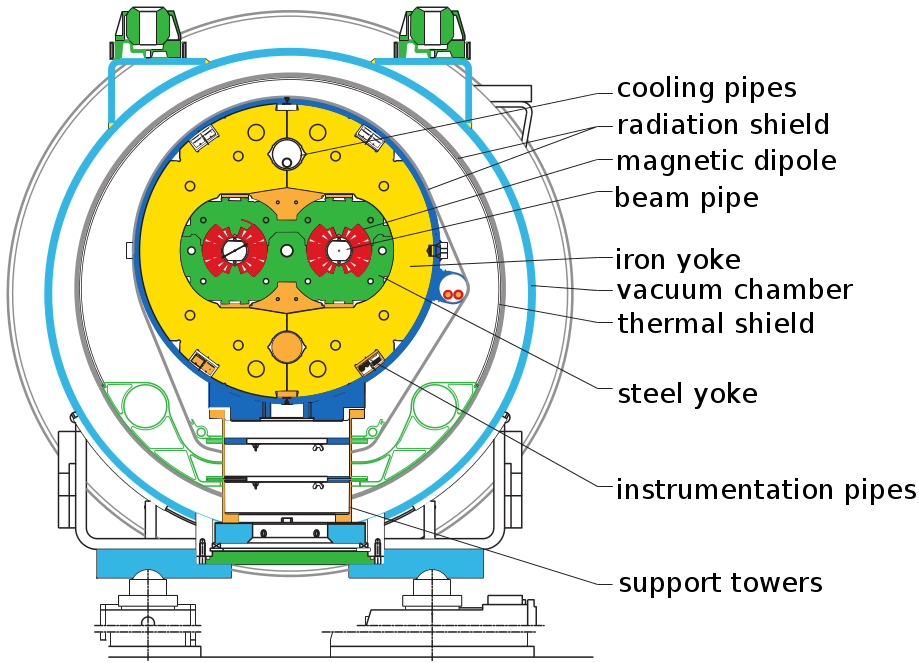
\includegraphics[scale=0.4]{ChapterCMS/figs/lhc_csp.png}
\source{BRUNING, 2017, p. 286. Adapted by the author.}
\label{fig:lhc_cs}
\end{figure}

The LHC operation was structured on the already existent accelerators at CERN. These accelerators are nowadays used to make the initial particle acceleration at smaller energies. The Tab.~\ref{fig:acel_compare} summarizes the energies and velocities achieved by a proton in each accelerator up to the LHC and Fig.~\ref{fig:LHC_parts} shows an scheme of the accelerators.

\begin{table}[htbp]{15cm}
\caption{Comparison between the energy and velocity achieved by a proton in the different accelerators located at CERN.}
\begin{tabular}{p{3cm}cc}
\hline \hline
Accelerator  & Kinetic energy (K)   & Velocity ($\%$c)	    \\
\hline
Linac 2		 & 50 MeV				& 31.4					\\
PS Booster	 & 1.4 GeV				& 91.6					\\
PS			 & 25 GeV				& 99.93 				\\
SPS			 & 450 GeV				& 99.9998				\\
LHC			 & 7 TeV				& 99.9999991			\\
\hline \hline
\end{tabular}
\source{CERN, 2008, p. 5.}
\label{fig:acel_compare}
\end{table}

At the LHC there are four main experiments (big detectors): ALICE (\textit{A Large Ion Collider Experiment}), ATLAS (\textit{A Toroidal LHC Apparatus}), CMS (\textit{Compact Muon Solenoid}), LCHb (\textit{Large Hadron Collider beauty}). These experiments are located on the beams collision points and each of them have a complex computing system, which the main frame is called Trigger system. The Trigger is responsible to combine the information coming from the sub-detectors in each experiment and identify the particles in a fast way in order to decide if a given event is interesting to be stored and further processed (in a more refined way). Such system is very important since, at 14TeVm the bunches composing the beams are spaced by 25~ns and generates $\sim$4*10$^{7}$ crossings every second, waht can lead up to $\sim$1~G events/s \cite{bib:JINST-3-362-2008, bib:lhc-guide}. In fact, there will be upgrades on this system for future collision scenarios as it is discussed at Appendix~\ref{app:cmsl1tt}.

\begin{figure}[htbp]{15cm}
\caption{Accelerators composing the LHC at CERN.}
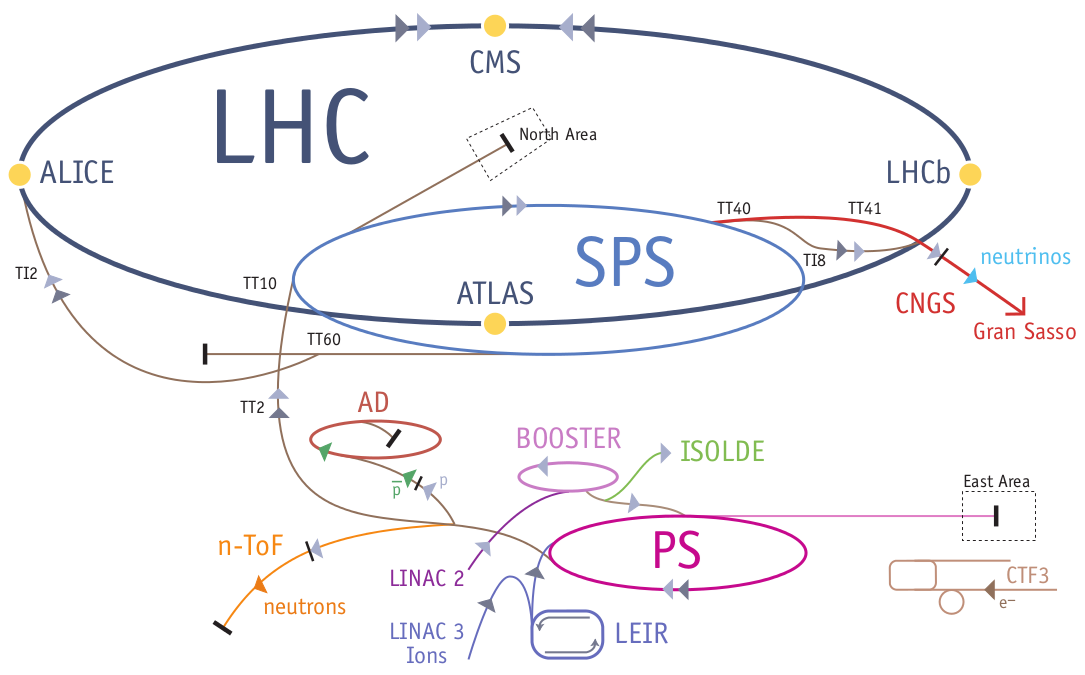
\includegraphics[scale=0.35]{ChapterCMS/figs/lhc_parts.png}
\source{CERN, 2008, p. 13.}
\label{fig:LHC_parts}
\end{figure}

\section{The CMS Experiment at the LHC}
The CMS is a general purpose experiment, which has similar physics goals as the ATLAS detector and both are used to look for different Physics topics. Different from ATLAS, the CMS has different detection techniques and a different magnetic system profile. Its construction is based on the traditional barrel model with two endcaps. As the name suggests, it was constructed to provide a good detection and resolution of muons. It has a giant cylindric coil made of super-conducting material, being able to generate a 3.8~T field (which is about 80 thousand times larger the the earth magnetic field). The CMS has 21~m of length, 15~m of diameter, weigh about 12500 tons and its construction cost is about R$\$$ 1,317 billions \cite{bib:lhc-guide,bib:cms-page}.

The construction of the CMS follows some requirements needed to the Physics goal in the TeV energy scale. Among them, is the good identification and resolution in the muons transverse momentum and charge, good reconstruction efficiency of the tracks from the tracker systems, good resolution in the energy deposited on the calorimeters and good resolution on the detection of missing transverse energy (MET).The coordinates system adopted in CMS has the origin in the beams collision point, while the 
\textbf{y} axis is in the vertical direction (positive to up) and the \textbf{x} axis points radially to the center of LHC circumference. Thus, the \textbf{z} axis is in the beams moving direction. The azimuthal angle $\phi$ is on the plane \textbf{xy}, being measured from the \textbf{x} axis and the polar angle $\theta$ is measured from the \textbf{z} axis. Usually, due to Lorentz invariance, the angle $\theta$ is replaced by the pseudorapidity which is defined as $\eta=-ln[tan(\theta/2)]$ \cite{bib:lhc-guide,bib:cms-page}.

The CMS experiment is composed by several sub-detectors distributed in radial layers (onion-like) around the beam pipe and each sub-detector is specialized in the detection of specific types of particles. The Fig.~\ref{fig:cms_fig1} show a sectioned view of the experiment and Fig.~\ref{fig:cms_fig2} how each type of particle interacts with each sub-detector. By combining the signals coming from each of those sub-detectors CMS collaboration uses a dedicated algorithm, called \textit{Particle Flow}, which reconstructs the particles by identifying the signals pattern across the entire CMS experiment. The main parts of the CMS are the tracker, the superconducting solenoid, the calorimeters, the muon chambers and the frontal detectors.

\begin{figure}[htbp]{16cm}
\caption{General view of CMS layers.}
\centering
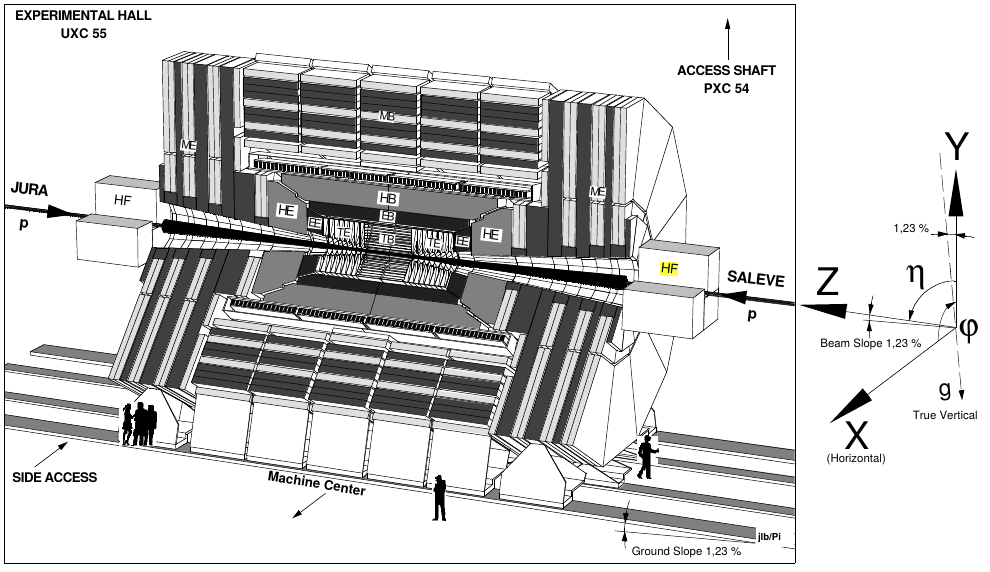
\includegraphics[scale=0.9,angle=90]{ChapterCMS/figs/cms_coordinates_system.png}
\source{CMS COLLABORATION, 2006, p. 5.}
\label{fig:cms_fig1}
\end{figure}

\begin{figure}[htbp]{16cm}
	\caption{Transverse section view showing the detection that each sub-detector does.}
	\centering
	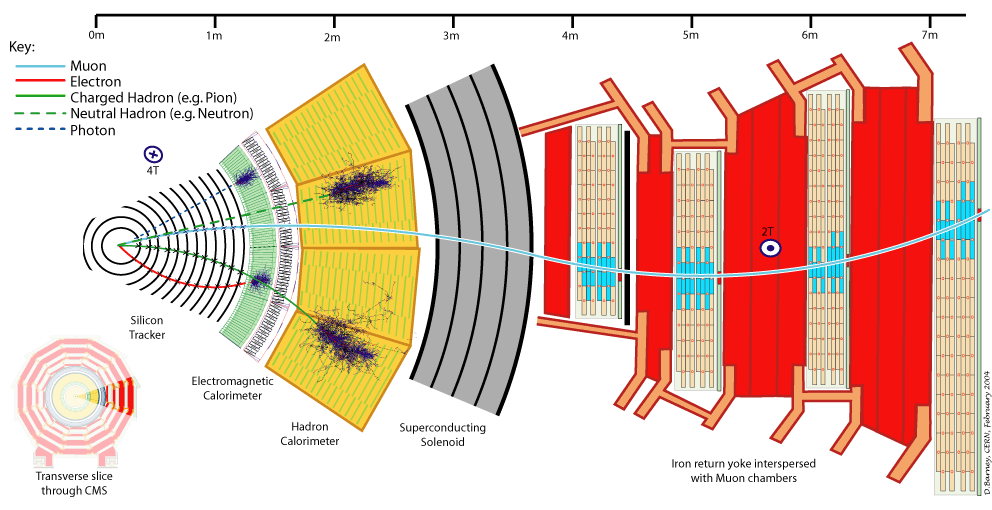
\includegraphics[scale=0.65,angle=90]{ChapterCMS/figs/cms_deteccao.png}
	\source{CMS, 2017.}
	\label{fig:cms_fig2}
\end{figure}

\subsection{The Tracker System}
The tracker system is composed by two set of detectors (Pixels and Strips) disposed radially around the beam pipe and has a total length of $\sim$5.40 m and total radius of $\sim$1.10 m. Each set presents a specific resolution but both of them detect the charged particles trajectory. The detectors used in the tracker are projected to support high radiation doses, since they are the ones closest to the collision point. Summing both set of detectors, the CMS tracker has $\sim$200 m$^{2}$ of active silicon ($SiO_{2}$). Its working principle is based on the ionization of silicon solid state sensors and in the collection of the generated charges by an electric field. These detectors stand out of the gas chambers due their higher density, which promotes absorption of higher energy particles \cite{bib:JINST-3-362-2008,bib:CMS-PTDR-2006,bib:grupen-2008}. Note, however, that this detector does not have the purpose to stop the particles, this is done by the calorimeters.

\subsubsection{The Silicon Pixels Detector}
The pixels detector comprehend the inner section of the tracker system and is projected to identify with high precision the particles trajectories in that region. It has great importance in the reconstruction of secondary vertices and in the measurement of small impact parameters, which are relevant for the identification of particles associated to heavy flavor quarks. This detector is composed by three cylindric layers, located around the beam pipe, and two discs (endcaps) located in the beam pipe transverse plane (Fig.~\ref{fig:pixel_detector}). The complete detector has 1~m$^{2}$ of silicon with 66 millions of pixels. The layers in the barrel extend for 53~cm and are disposed radially at 4.4, 7.3, 10.2~cm from the \textbf{z} axis. In the barrel there are 768 pixels with area 100$\times$150~$\mu$m$^{2}$ and disposed in a half-stair fashion way. In the discs exist 672 pixels disposed in helice and rotated by 20$^{\circ}$ around the radial direction. The pixel detector has a coverage of $|\eta| < 2.5$ and presents a resolution of about 10~$\mu$m in the \textbf{r-$\phi$} and 20~$\mu$m in the \textbf{z} direction.

\begin{figure}[htbp]{15cm}
\caption{Scheme of the pixel detector.}
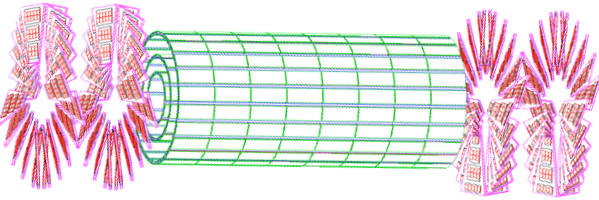
\includegraphics[scale=0.5]{ChapterCMS/figs/pixel_detector.png}
\source{CMS COLLABORATION, 2006, p. 20.}
\label{fig:pixel_detector}
\end{figure}

\subsubsection{The Silicon Strips Detector}
The silicon strips detector is the tracking system positioned around the pixels detector, being divided into two parts identified as: the Tracker Inner Barrel (TIB) and the Tracker Outer Barrel (TOB). The TIB is composed by four layers of silicon sensors with thickness of 320~$\mu$m and cover the region for $|\textbf{z}| < 65$~cm. The TOB has 6 layers, also of $SiO_2$, with average length of $|\textbf{z}| < 110$~cm. The silicon strips detector also has endcaps, which are divided into two categories: Tracker EndCaps (TEC) and Tracker Inner Discs (TID). Each TEC is composed by 9 discs which are disposed in the region $120 < |\textbf{z}| < 280$~cm and each TID is composed by 3 small discs which fill the space between the TIBs and the TECs. Both TID and TEC are organized in rings around the beam pipes and the sensors that constitute them have thickness of 320~$\mu$m (the entire TID and the 3 inner layers of the TEC) and 500~$\mu$m (remaining TEC layers). This entire detector has the length of 5.8 m and diameter of 2.6 m, containing about 10 million $SiO_{2}$ fibers. Its main designation is the track reconstruction from muons, isolated electrons and charged hadrons with high transverse momentum, keeping an efficiency higher than 98$\%$ in the interval $|\eta| < 2.5$.

\subsection{The Calorimeters}
A calorimeter is a system in which the particles are totally absorbed in order to measure their energy, that is, the particle is stopped. There are two types of calorimeters in the CMS: the Electromagnetic Calorimeter (ECAL) and the Hadronic Calorimeter (HCAL). The ECAL is designed to measure the energy of particles which interacts mainly electromagnetically with its material, such as electrons and photons. At high energy, the electrons lose their energy almost exclusively by the \textit{bremsstrahlung} process. The photoelectric and Compton effects also happen. The HCAL is built to measure the energy of particles which interact through the strong and weak interactions, the case of hadrons such as pions, kaons and so on. The particles interacting with the calorimeters usually produce showers of other particles which appear from the decay of the first ones. The precision on the measurement of the energy deposited in a calorimeter is given by $\Delta E/E \propto 1/ \sqrt{E}$, and thus, the LHC can measure the particles energy with higher precision than the previous colliders.

\subsubsection{The Electromagnetic Calorimeter (ECAL)}
The ECAL is a hermetic\footnote{Capable to detect all the products of a decay by covering a big area around it (in other words, maximum coverage in the solid angle).} and homogeneous calorimeter, composed by 61200 $PbWO_4$ crystals disposed over the central barrel (EB) and by 7324 crystals in each endcap (EE). Among the properties which lead to the choice of the $PbWO_4$ as the material for the calorimeter scintillators, are the short radiation wave length ($\chi=0.89$~cm) and the short Molière radius (2.2~cm). This allowed the construction of a compact calorimeter. The Molière radius is a radial measurement of a cylinder, around the shower axis, which contains about 95$\%$ of its total energy, being almost independent of the energy of the incident particle. Additionally, the $PbWO_4$ scintillators are fast such that about 80$\%$ of the produced light is emitted in the interval of 25 ns \cite{bib:JINST-3-362-2008,bib:grupen-2008}.

In the barrel, the ECAL-EB covers a region of $|\eta| < 1.479$, with granularity of 1 crystal for each 1$^{\circ}$ in $\phi$. These crystals measure 23 cm in length and have faces with 22$\times$22~mm$^{2}$ (front) e 26$\times$26~mm$^{2}$ (back, where the photo-multipliers are coupled), forming a total volume of 8.14 m$^{3}$ (and weighting 67.4 tons). The $PbWO_4$ crystals are supported by a aluminum structure that keeps them spaced from each other by 0.35 mm and grouped in sub-modules. Such sub-modules are grouped in modules containing from 400 to 500 crystals. Finally, a trapezoidal structure groups four modules in so called super-modules, which form a half angular section of the barrel containing 1700 crystals (Fig.~\ref{fig:ecal}). In order to form half arc of the barrel, 18 super-modules are needed, each covering 20$^{\circ}$. On each sub-module the crystals are positioned forming a small angle with respect to the collision point in order to have coincidence between the crystal axis and the radial axises from the coordinate system.

The ECAL endcaps cover a region with $1.479 < |\eta| < 3.0$ and are installed 314 cm away from the CMS coordinates system.In that region the endcap is composed by crystals grouped in 5$\times$5 unities (called super-crystals or SCs) by a structure made of carbon fiber. Each crystal has 22 cm in length and present faces of 8.4 cm$^{2}$ (front) and 9 cm$^{2}$ (back). On each endcap, the ECAL is divided in two halves (called \textit{Dees}) which contain 3662 crystals each one. The crystals and the SCs are organized in a rectangular grid (\textbf{xy}) pointing to the origin of the CMS coordinates system. The two endcaps together comprehend a volume of 290 cm$^{3}$ and weigh 24 tons. In front the scintillators, on each endcap, there is also a shower detector (called \textit{preshower}). This detector is composed of two planes of silicon trips. The main goal of the preshower is to identify neutral pions in the region $1.653 < |\eta| < 2.6$, which allows the suppression of significant backgrounds in the $H \rightarrow \gamma\gamma$ channel \cite{bib:JINST-3-362-2008,bib:CMS-PTDR-2006}.

\begin{figure}[htbp]{15cm}
\caption{Illustration of a super-module and the entire ECAL.}
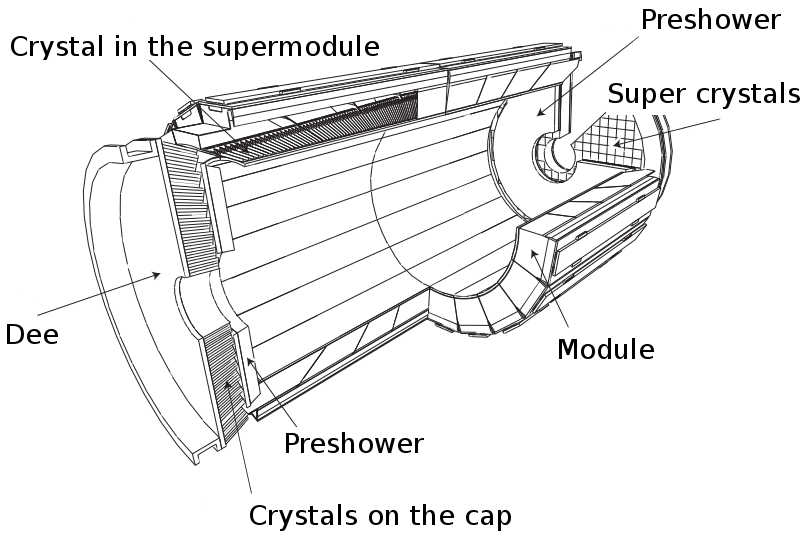
\includegraphics[scale=0.4]{ChapterCMS/figs/ecal_sched.png}
\source{CMS COLLABORATION, 2008, p. 93 and 95. Adapted by the author.}
\label{fig:ecal}
\end{figure}

\subsubsection{The Hadronic Calorimeter (HCAL)}
Hadronic calorimeters are particularly important to the detection of jets and particles that lead to unbalance of the total energy (MET). The HCAL is installed around the ECAL in the CMS and its profile was strongly guided by the behavior of the magnetic field (since the biggest part of the HCAL is inside the solenoid). An important requirement for this detector is the enhancement on the resolution of the energy deposited on it and provide good hermecity for correct measurement of MET. This is achieved by the addition of an extra layer positioned after the solenoid, such that, the CMS HCAL can be divided in three parts: the barrels inside (HB~-~\textit{Hadron Barrel}) and outside (HO~-~\textit{Hadron Outer}) of the solenoid and, the endcaps (HE~-~\textit{Hadron Endcap}). In the barrel the HCAL goes radially from the ECAL ($R = 1.77$ m) up to the solenoid ($R = 2.95$~m).

The HB is composed by 36 towers divided in two halves with respect to the \textbf{z} axis (Fig.~\ref{fig:hcal_hb}) and covers the region with $|\eta|<1.3$. The towers are made of absorbent brass, constituted of 70$\%$ of Cu and 30$\%$ of Zn (density of 8.53~g/cm$^{3}$). There are inner and outer plates made of stainless steel that holds the towers. The complete HB towers have, then, the following structure: a steel plate with thickness of 4 cm, followed by eight brass plates with thickness of 5.1 cm and six brass plates of 5.7 cm, finishing with another steel plate with 7.5 cm. The effective HB thickness increases with the polar angle (since the particle trajectory increases) and the presence of the ECAL before the HCAL adds about 1.1~$\lambda_I$ de material \cite{bib:JINST-3-362-2008,bib:CMS-PTDR-2006}.

\begin{figure}[htbp]{15cm}
\caption{Scheme of the positions of the HB towers.}
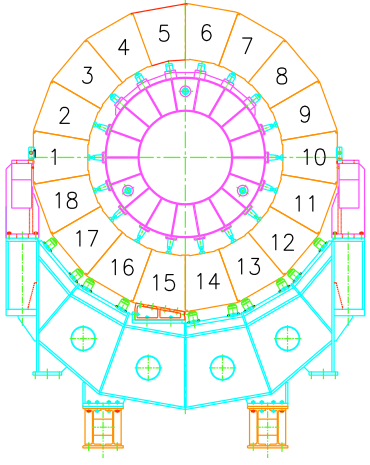
\includegraphics[scale=0.4]{ChapterCMS/figs/hcal_hb.png}
\source{CMS COLLABORATION, 2008, p. 125.}
\label{fig:hcal_hb}
\end{figure}

The HE covers a region with $1.3 < |\eta| < 3$, which contains in general about 34$\%$ of the particles produced as final states. The material used on its construction was constrained by the conditions of high luminosity, the capacity of high rates counting and the high magnetic field. The chosen material for this detector was the so called C26000, which is a compound also based in brass. Each HE is coupled to the support of the muon detection system in the CMS endcaps and constitutes 36 towers positioned behind the EE (Fig.~\ref{fig:hcal_he}). The geometry used in the HE construction has the goal to reduce the discontinuities between it and the HB, besides aiming a better energy resolution of a single particle. The used brass plates have thickness of 7.9 cm and present between them plastic scintillators with $\sim$9 mm.

\begin{figure}[htbp]{15cm}
\caption{Scheme of the hadronic calorimeter in the endcaps, annexed to the muon detection system.}
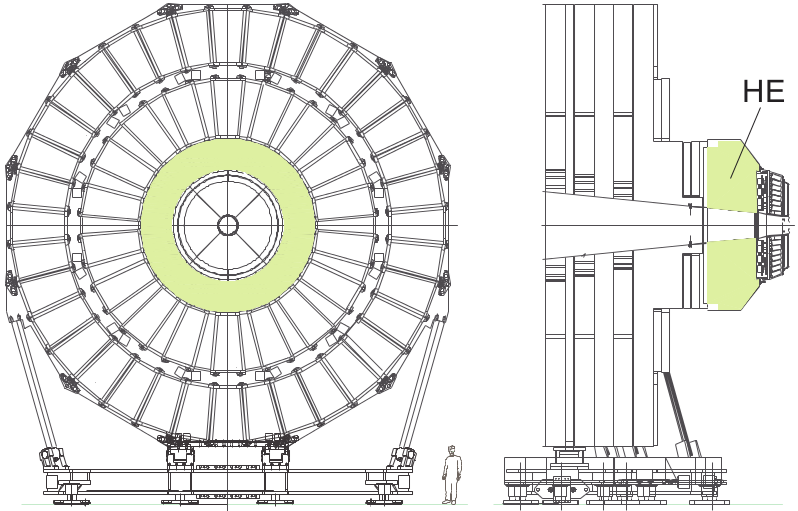
\includegraphics[scale=0.4]{ChapterCMS/figs/hcal_he.png}
\source{CMS COLLABORATION, 2008, p. 131.}
\label{fig:hcal_he}
\end{figure}

Because of the radial limitation associated to the solenoid there is an additional HCAL layer positioned behind it. This is needed since the combined absorption power of the EB and the HB is not enough to fully handle some hadronic showers. The HO covers a region of $|\eta| < 1.3$ and uses the solenoid as additional material, being able to detect showers with retarded start and thus, the reminiscent energy after the HB. The physical impact of the HO has been studied in CMS simulation. Without it one observes an excess in the ratio E$_{measured}$/E$_{incident} < 1$ (Fig.~\ref{fig:hcal_ho_sim}), which means that, part of the total energy is lost in the reconstruction (showers "leakage" - the showers are not completely reconstructed). Such effect has a direct impact on the measure of MET and thus, the HO is an important detector for the study of processes involving strong interactions \cite{bib:JINST-3-362-2008,bib:hcal-tdr-1997}.

\begin{figure}[htbp]{15cm}
\caption{Scheme of the positions of HO in the muon detection systema and its effect on the measurement of the energy from hadronic showers.}
\subfloat[HO transverse section.]{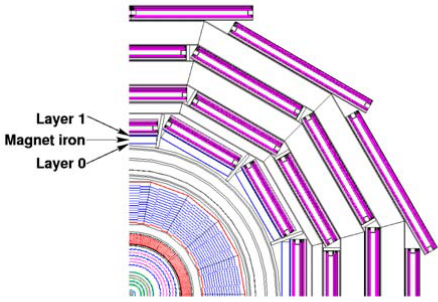
\includegraphics[scale=0.7]{ChapterCMS/figs/hcal_ho.png}} \hspace{0.5cm}
\subfloat[HO effect on the balance of energy measured in the CMS.]{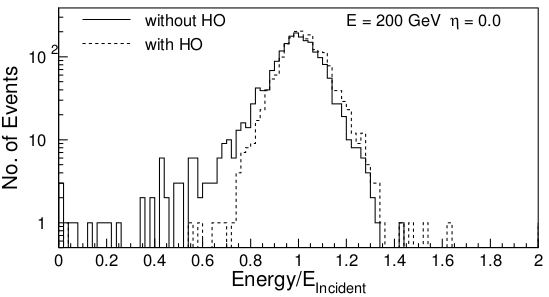
\includegraphics[scale=0.6]{ChapterCMS/figs/ho_sim.png}}
\source{CMS COLLABORATION, 2008, p. 138 and 140.}
\label{fig:hcal_ho}
\label{fig:hcal_ho_sim}
\end{figure}

In the forward CMS directions there are also the HFs (Hadron Forward detectors). The HFs are calorimeters which receives very high fluxes of particles (on average 760 GeV per pp interaction is deposited into the two forward calorimeter - very large compared to the 100 GeV for the rest of CMS). Also, such energy is not uniformly distributed but increases with higher pseudorapidities. The HFs are essentially a cylindrical steel absorber structure composed by 5 mm thick grooved plates. Quartz Optical fibers are inserted in such grooves. The detector is functionally divided into two longitudinal segments. Half of the fibers run over the full depth of the absorber (165 cm) while the other half starts at a depth of 22 cm from the front of the detector. These two sets of fibers have separated read out systems. Such arrangement makes it possible to distinguish between showers generated by electrons and photons (which deposit a large fraction of their energy in the first 22 cm), from the showers generated by hadrons (which produce nearly equal signals in both calorimeter segments). The HFs are located at about 11.2 m from the collision point and their inner radius is at 12.5 cm from the beam line center. The outer radius goes up to 130.0 cm. The total coverage of the HFs comprehend the region $3.0 < |\eta| < 5.0$ \cite{bib:JINST-3-362-2008,bib:hcal-tdr-1997}. Fig.~\ref{fig:hcal_hf} shows a scheme of a quadrant of the HF detector and the grooves where the optical fibers sit.

\begin{figure}[htbp]{15cm}
	\caption{An HF quadrant showing the modules of steel plates with grooves where optical fibers sit.}
	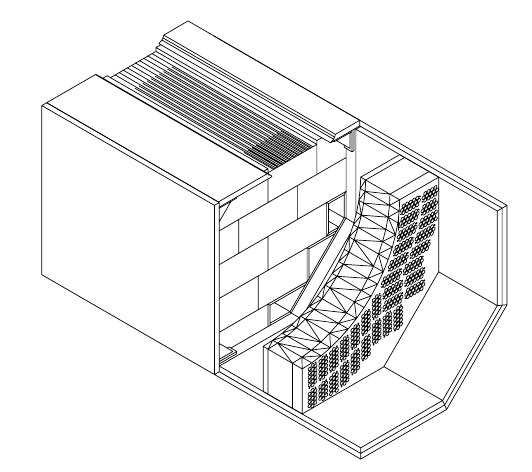
\includegraphics[scale=0.5]{ChapterCMS/figs/hcal_hf.png}
	\source{CMS COLLABORATION, 1997, p. 138 and 140.}
	\label{fig:hcal_hf}
\end{figure}


\subsection{The Magnetic System}
The CMS magnetic system has the main goal the efficiency in the detection muon system and thus, also the power to bend such particles in the momentum range of $\sim$1 TeV in order to distinguish their charge. That requires a resolution of $\Delta p/p \sim10\%$ at this given momentum. For this reason, the CMS Collaboration choice was a big superconducting solenoid with 12.9 m of length, consisting of 5 rings of 5.9 m of inner radius (Fig.~\ref{fig:cms_solenoid}). Because of the huge number of wire turns needed to achieve the required magnetic field, the solenoid coil is composed by 4 layers, differing from the usual one and two layers, as for Aleph and Delphi and, ZEUS and BaBar experiments, respectively. In total CMS has 2168 wire turns. The solenoid and the wires are made of NbTi and aluminum of high purity. Due to the huge magnetic field, a big part of the solenoid has structural functionality.

Because of physical reasons the radial extension of the solenoid is relatively small ($\Delta R/R \sim 0.1$) but even so, its mass is about 220 tons and it can holds up to 2.6 GJ of energy. In order to keep the solenoid superconducting a huge cryogenic system is needed. This system was constructed with a cooling capacity of 800 W at 4.45 K and 4500 W between 60-80 K and, simultaneously for a liquefaction capacity of 4 g/s. Associated to it, there is also a vacuum system capable of produce good isolation for a volume of 40 m$^{3}$. In order to assure the return of the magnetic field generated by the solenoid, a big structure made of iron (\textit{yoke}) is used in the external region around the solenoid. Such structure is composed of 11 big sections: 6 discs (endcaps) and 5 cylinders (barrel region), with masses that vary between 400 and 1920 tons. For a precise moving of such structures (during the CMS maintenances, for instance), they sit over platforms that float over air or oil (\textit{heavy-duty air pads} and \textit{grease pads}). Because of this system the alignment of the parts composing the \textit{yoke} was done in such a good way that the final accuracy was of 2 mm of difference from the ideal center (the center of the coordinates system) \cite{bib:JINST-3-362-2008}.

\begin{figure}[htbp]{15cm}
\caption{The CMS magnetic system.}
\subfloat[Scheme of the CMS solenoid.]{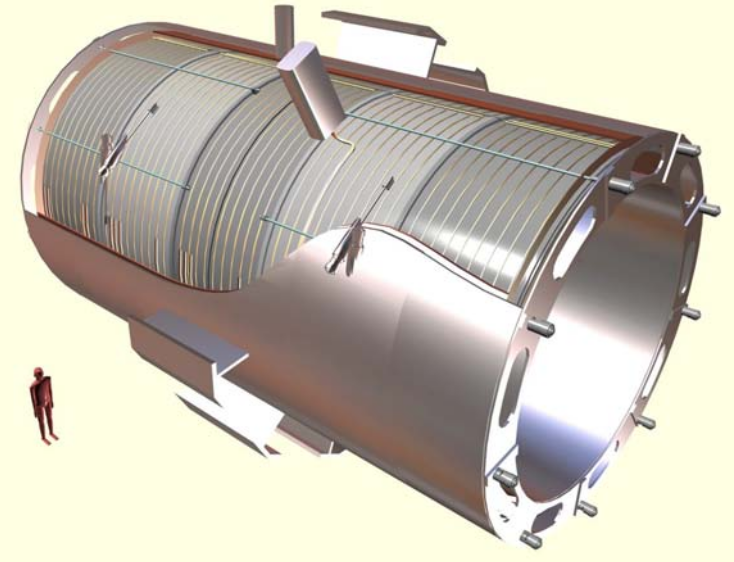
\includegraphics[scale=0.5]{ChapterCMS/figs/solenoid.png}}\quad
\subfloat[Mapping of the magnetic field created by the solenoid.]{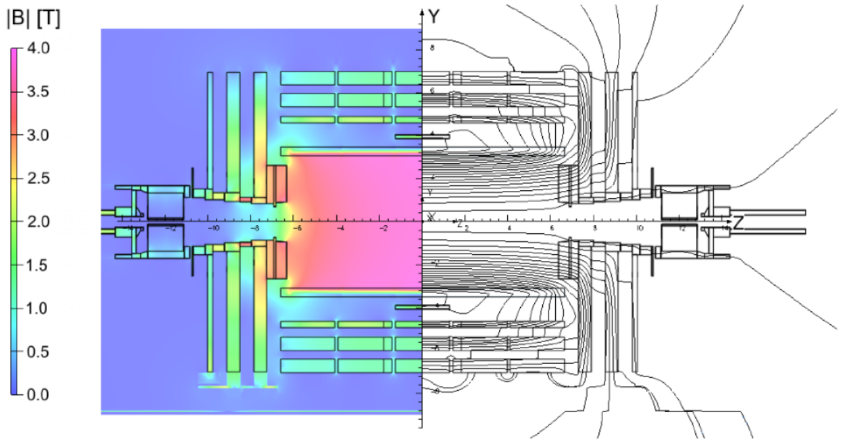
\includegraphics[scale=0.65]{ChapterCMS/figs/cms_magnetic_field_map}}
\source{CMS COLLABORATION, 2008, p. 7.}
\label{fig:cms_solenoid}
\end{figure}

\subsection{The Muon Chambers}
This is the last and outermost set of detectors in the CMS experiment. It is constituted of 4 radial stations inserted in cavities of the \textit{yoke} and is responsible for the identification and the measure of the transverse momentum of muons. The muon chambers are divided in three categories: the drift tube chambers (DTCs), the Cathode Strip Chambers (CSCs) and the Resistive Plate Chambers (RPCs). The DTCs are located in the barrel region, while the CSCs in the endcaps and the RPCs are installed in both barrel and endcaps. Such detectors covers the region of $0 < |\eta| < 2.4$. In the barrel the DTs cover $0 < |\eta| < 1.3$ while in the endcaps the CSCs cover $0.9 < |\eta| < 2.4$. The measurement of the muons transverse momentum using only the muon chambers is determined essentially by the curvature angle of the muons coming out of the solenoid and is not efficient as the tracker system. However, the combination of the tracker with the muon chambers can increases the resolution on the transverse momentum measurement by a factor of up to 10x (Fig.~\ref{fig:preso_detectors}) \cite{bib:CMS-PTDR-2006,bib:CMS-MSTDR-1997}.

\begin{figure}[htbp]{16cm}
\caption{Comparison of the resolution on the muon transverse momentum measurement obtained by using the muon chambers and the tracker separated and combined, left. Scheme of the muon chambers position in the CMS, right}
\centering
\subfloat[Resolutions on the measruement of the muons transverse momentum.]{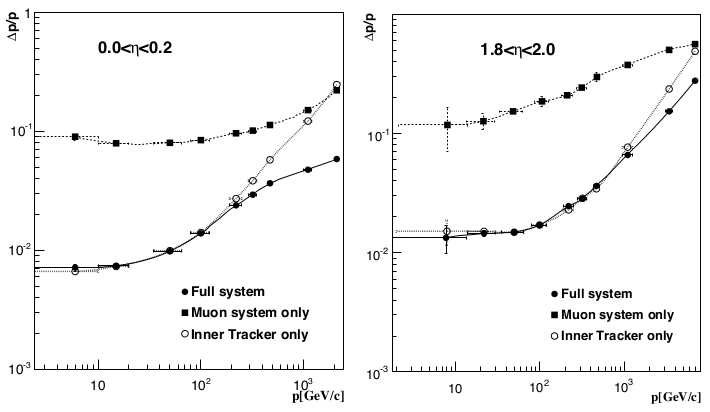
\includegraphics[scale=0.6]{ChapterCMS/figs/pmu_reso.png}}\\
\subfloat[Location of the muon chambers in a section of the CMS detector.]{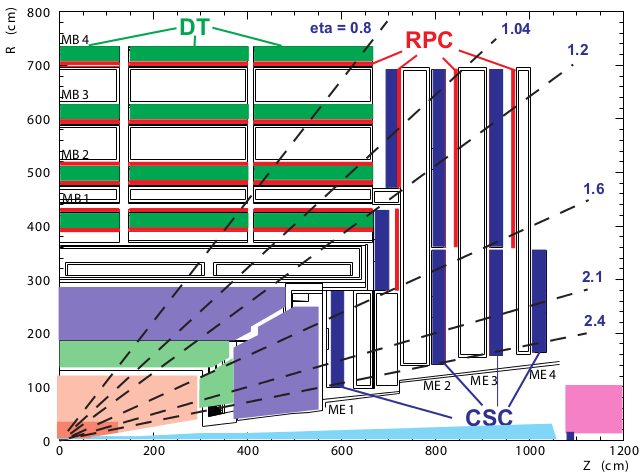
\includegraphics[scale=0.6]{ChapterCMS/figs/sist_muon_position.png}}
\source{CMS COLLABORATION, 2006, p. 11 and 12.}
\label{fig:preso_detectors}
\end{figure}

In the CMS barrel region, the muon chambers are composed by 4 stations that form concentric cylinders positioned radially at 4.0, 4.9, 5.9 and 7.0 m of the beam line center (totalizing 250 chambers). The geometry of the \textit{yoke} presents 12 sectors covering 30$^{\circ}$ in \textbf{$\phi$} and the chambers are disposed in such a way that a high momentum muon produced close to the borders of adjacent sectors crosses at least 3 or 4 chambers. There are 12 chambers in each of the 3 inner stations, while in the fourth station, the sectors above and below (hemispherically) hold 2 chambers. Each station was designed to produce a spacial vector associated to the muons with a precision em \textbf{$\phi$} better than 100 $\mu$m. The muon chambers in the endcaps is constituted of 468 CSCs in trapezoidal shape and are superposed between each other, covering the full azimuthal region (orthogonal to the beam axis). The chambers in that region has thickness of 60-10 cm, and each one covers about 10$^{\circ}$ (radially outer chambers) and 20$^{\circ}$ (radially inner chambers). All RPCs installed in the endcaps cover 20$^{\circ}$.

Although there are structural differences between the technologies used in each type of chamber, all of them work in similar way (cathode-anode principle). The DTCs are made of tubes containing gas ($Ar+CO_2$) in which there is a conducting wire Fig.~\ref{fig:sist_muon_detectors}(a). A potential difference created between the tube and the wire creates electric field such that, any charged particle crossing the tube ionizes the gas and produces a bunch of electrons (which can produce even more electrons - avalanche process) that are drifted to the wire and produces an excess of current in the detector (the signal). The distance between the particle and the wire is a function of the velocity and the time associated to the electrons in order to achieve the wire. Each DTC is composed of 12 layers of aluminum organized in 3 groups of 4, containing up to 60 tubes each one. Each layer measures in average 2$\times$2.5~m$^{2}$ and each tube is 4 cm wide. The CSCs consist of wires perpendicularly positioned to cooper fibers inserted in a gas Fig.~\ref{fig:sist_muon_detectors}(c). The difference from the DTCs are basically the higher resolution due to the use of cathodes in strip shape, which allows higher precision on the estimation of the electrons avalanche position. The RPCs are detectors composed by two parallel plates made of a plastic material with high electric resistivity and separated by gas Fig.~\ref{fig:sist_muon_detectors}(b). The plates are transparent to the electrons generated in the ionization process and those are collected by metallic fibers located after the plates. RPCs are detectors that combine a good spatial and temporal (1 ns) resolution and, because of that they are used to trigger the presence of particles in the muon detection system \cite{bib:CMS-PTDR-2006,bib:CMS-MSTDR-1997,bib:grupen-2008}.

\begin{figure}[htbp]{16cm}
\caption{Types of detectors used in the muon detection system.}
\begin{multicols}{2}
\subfloat[DTC scheme.]{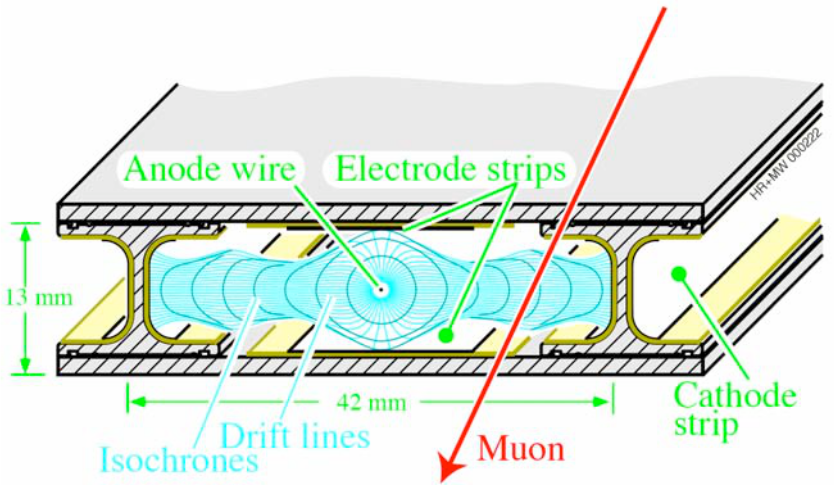
\includegraphics[scale=0.23]{ChapterCMS/figs/dtc.png}}\\
\subfloat[RPC scheme.]{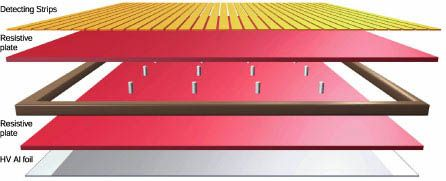
\includegraphics[scale=0.44]{ChapterCMS/figs/rpc.jpg}}\\
\subfloat[CSC scheme.]{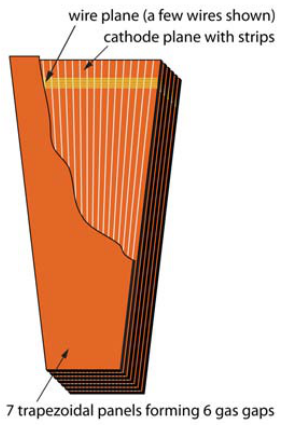
\includegraphics[height=7cm,width=5.5cm]{ChapterCMS/figs/csc.png}}
\end{multicols}
\source{CMS COLLABORATION, 2008, p. 169 and CMS COLLABORATION, 2006, p. 94.}
\label{fig:sist_muon_detectors}
\end{figure}


\subsection{The Trigger and Data Acquisition System}
The trigger system and data acquisition (TriDAS~-~\textit{Trigger and Data Acquisition System}) in a hadronic collider has a very important function, since, both the collision rates and the amount of data produced are much larger than the speed and size which can be handled. At the LHC, about 1.5 MB of data can be produced per event during the crossing of the proton bunches. In such way a system that reduces the amount of data at the moment of the collision is needed. Much of what is produced in the LHC is already known Physics and very efficient filters need to be applied in order to store the Physics potentially new. Since the event rate is very high ($\mathcal{O}(10^{6})$), the filtering is divided into two stages: the level-1 trigger (L1T) and the high level trigger (HLT) \cite{bib:JINST-3-362-2008,bib:CMS-DAS-TDR-2002}. 

The L1T is composed by custom programmed hardware in (or very close to) the sub-detectors and is designed to reduce the event rate to 100 kHz. This trigger can be divide into local, regional and global components, which use informations coming from calorimeters and muon chambers to identify and organize specific objects (\textit{trigger object} - such as the EG candidates) according to their energy/momentum and the quality of such informations (which constitutes the confidence level). In 2016 there was a list (L1 trigger menu) of about 200 requirements (L1 seeds), which constitute specifications that an event should satisfy. In order to be forward for further analysis, an event has to fire the L1 seeds. If that happens then the event is sent to the next level, the HLT \cite{bib:JINST-3-362-2008,bib:CMS-DAS-TDR-2002}.

The HLT is a more complex filter based on pure software. It filters the events using a set of algorithms running on a computer farm. These algorithms are a simplified version of the algorithms used for event offline reconstruction. The HLT is designed to reduce the event rate to 100 Hz. In order to be stored an event needs to satisfy at least one of the HLT requirements (trigger paths). When that happens the event is marked for permanent storage and it is transferred to the CERN T0. Once an event is triggered by the HLT and stored in the CERN T0 it follows to the full event reconstruction. This processing is done offline (no time constraints) using the complete resolution and full information of the CMS sub-detectors and, takes at least 48h to be complete. After that, the event is ready for Physics analysis \cite{bib:JINST-3-362-2008,bib:CMS-DAS-TDR-2002}.